\chapter{Осцилляторы, числа заполнения и первое квантовое поле}

Квантовая теория поля — это наш базовый формализм для практически всей известной негравитационной физики. Это утверждение не следует путать с утверждением, будто любую задачу можно решить. Атом водорода поддаётся рассмотрению; когда мы переходим к атому вроде бора, вычисление уже становится намного труднее, а человек находится далеко за пределами любых реалистичных вычислений в теории поля. Формализм может быть фундаментальным, тогда как его уравнения остаются подавляюще трудными.

Поэтому мы войдём в предмет самым элементарным возможным способом. Эту область иногда называют \emph{вторичным квантованием}, но само название мало что скажет, пока мы не построим нужный аппарат. Кратчайший путь начинается не с релятивистского поля, а с гармонического осциллятора. Пружины здесь не главное. Важна алгебра операторов повышения и понижения. Когда эта алгебра повторяется для многих мод, оператор повышения перестаёт означать просто ``поднять осциллятор на один уровень'' и начинает буквально означать ``создать частицу.''

\section{Осциллятор как алгебра}

Для одного осциллятора пусть \(a^\dagger\) повышает возбуждение, а \(a\) понижает его. Обозначения \(a_+\) и \(a_-\) равносильны, но запись с кинжалом предвосхищает язык, используемый в теории поля. Нижайшее состояние удовлетворяет
\begin{equation}
a|0\rangle=0,
\end{equation}
а оператор числа имеет вид
\begin{equation}
N=a^\dagger a,
\qquad
N|n\rangle=n|n\rangle.
\end{equation}
Эти два лестничных оператора эрмитово сопряжены друг с другом, и их основной коммутатор равен
\begin{equation}
[a,a^\dagger]=1.
\label{eq:l06-single-commutator}
\end{equation}
Эта небольшая алгебра почти исчерпывает всё содержание осциллятора.

Операторы \(a\) и \(a^\dagger\) можно получить как подходящие линейные комбинации координаты и импульса. Точное соглашение зависит от нормировки \(x\), \(p\), \(m\) и \(\omega\); полезное инвариантное утверждение здесь состоит в том, что \(a^\dagger a\) восстанавливает квадратичный гамильтониан осциллятора с точностью до аддитивной энергии основного состояния. Поэтому
\begin{equation}
H=\hbar\omega\left(N+\frac12\right).
\end{equation}
В дальнейшем обсуждении мы отбросим постоянный член и будем работать с
\begin{equation}
H=\hbar\omega N.
\label{eq:l06-one-oscillator-hamiltonian}
\end{equation}
Частота задаёт цену одного возбуждения. Увеличение \(n\) на единицу стоит \(\hbar\omega\); уменьшение \(n\) на единицу высвобождает ту же величину.

\section{Множество независимых осцилляторов}

Теперь рассмотрим много осцилляторов и занумеруем их индексом \(i\). Это обозначение — лишь индекс, а не мнимая единица. Число мод может быть конечным или бесконечным. Наглядной моделью может служить набор независимых пружин; другой — нормальные моды идеальной скрипичной струны. В приложениях теории поля важен именно бесконечный набор.

Независимость имеет операторный смысл. Операторы, относящиеся к действительно независимым подсистемам, коммутируют. Иначе соответствующие величины нельзя было бы измерять независимо, и сами системы изначально не были бы независимыми. Поэтому имеем
\begin{align}
[a_i,a_j]&=0, \\
[a_i^\dagger,a_j^\dagger]&=0, \\
[a_i,a_j^\dagger]&=\delta_{ij}.
\label{eq:l06-many-commutators}
\end{align}
При \(i\ne j\) всё, относящееся к этим двум модам, коммутирует. При \(i=j\) последняя строка сводится к уравнению~\eqref{eq:l06-single-commutator}.

У каждого осциллятора есть свой оператор числа и, вообще говоря, своя частота:
\begin{equation}
N_i=a_i^\dagger a_i,
\qquad
H=\sum_i\hbar\omega_i N_i.
\label{eq:l06-many-hamiltonian}
\end{equation}
Одновременное собственное состояние задаётся полным списком
\begin{equation}
|n_1,n_2,n_3,\ldots\rangle,
\qquad n_i=0,1,2,\ldots.
\label{eq:l06-occupation-ket}
\end{equation}
Целое число \(n_i\) называется \emph{числом заполнения} \(i\)-го осциллятора. На этом этапе это лишь термин. Вскоре оно будет считать частицы, занимающие одночастичное состояние, и название станет буквальным.

Состояние, в котором все числа заполнения равны нулю, имеет вид
\begin{equation}
|0\rangle\equiv|0,0,0,\ldots\rangle,
\qquad a_i|0\rangle=0\quad\text{for every }i.
\label{eq:l06-oscillator-vacuum}
\end{equation}

\begin{classroomqa}
\lecturetimestamp{00:15:27}
\audiencequestion{Соответствует ли бесконечное семейство осцилляторов континууму мод системы вроде скрипичной струны?}
\lecturerresponse{Да, для идеализированной струны. Реальная струна состоит из атомов, поэтому достаточно короткие длины волн в конце концов натыкаются на микроскопическое отсечение. Тем не менее модель сплошной среды мотивирует бесконечный набор мод, используемый в теории поля.}
\end{classroomqa}

\section{Почему коэффициенты лестничных операторов — квадратные корни}

Действие \(a^\dagger\) должно переводить собственное состояние оператора \(N\) в следующее собственное состояние, но нормировка допускает коэффициент:
\begin{equation}
a^\dagger|n\rangle=c_n|n+1\rangle.
\label{eq:l06-unknown-coefficient}
\end{equation}

\begin{figure}[htbp]
\centering
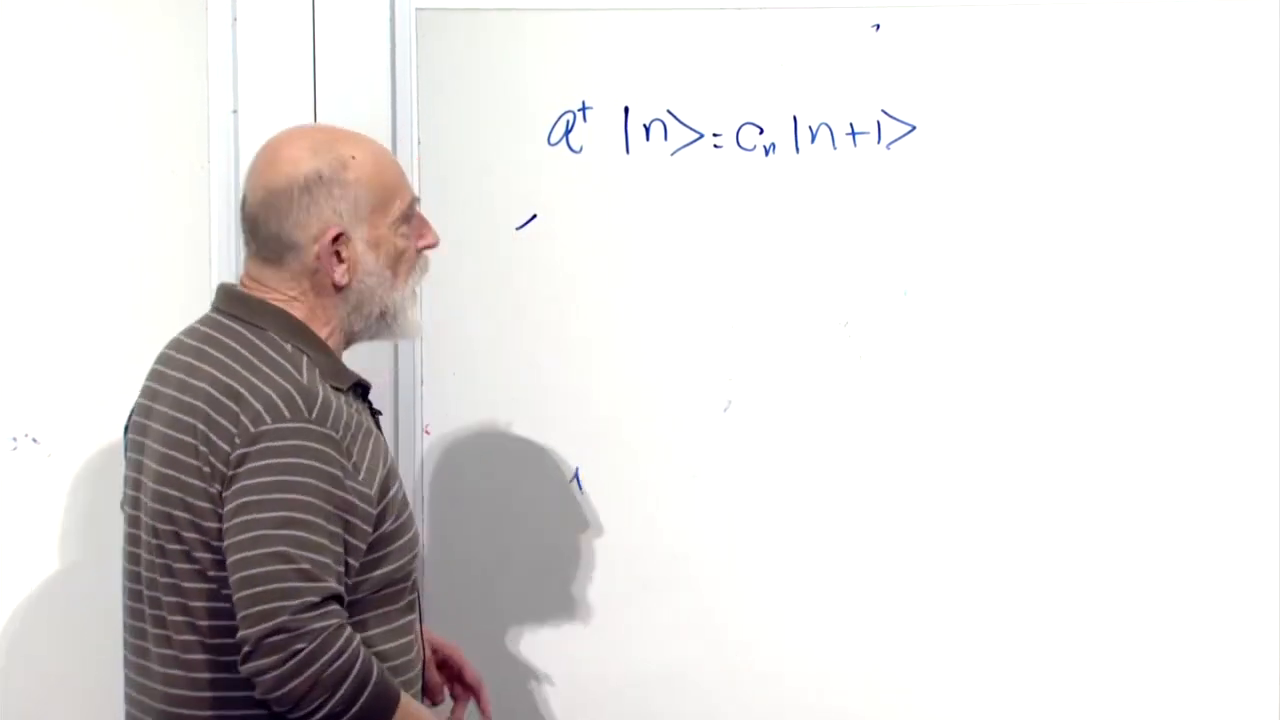
\includegraphics[width=0.9\linewidth]{lecture_06_frame_01.png}
\caption{Коэффициент лестничного оператора вводится до вывода его нормировки. Уравнение, написанное на доске, воспроизведено в уравнении~\eqref{eq:l06-unknown-coefficient}.}
\lectureframe{00:19:38}
\end{figure}

Выберем фазовое соглашение, в котором \(c_n\) вещественно. Переход к эрмитову сопряжению даёт
\begin{equation}
\langle n|a=c_n\langle n+1|.
\end{equation}
Умножая эти два соотношения и используя нормированные базисные состояния, получаем
\begin{align}
c_n^2
&=\langle n|aa^\dagger|n\rangle \\
&=\langle n|(a^\dagger a+1)|n\rangle \\
&=\langle n|(N+1)|n\rangle \\
&=n+1.
\end{align}
Следовательно,
\begin{equation}
a^\dagger|n\rangle=\sqrt{n+1}\,|n+1\rangle.
\label{eq:l06-raising-rule}
\end{equation}

\begin{classroomqa}
\lecturetimestamp{00:22:35}
\audiencequestion{Почему можно положить \(\langle n+1|n+1\rangle=1\) ещё до нахождения \(c_n\)?}
\lecturerresponse{Собственные векторы с самого начала выбираются как нормированный базис. Их нормировка не определяет нормировку \(a^\dagger|n\rangle\); именно эта оставшаяся информация и содержится в коэффициенте \(c_n\).}
\end{classroomqa}

Правило понижения получается тем же способом:
\begin{equation}
a|n\rangle=\sqrt n\,|n-1\rangle.
\label{eq:l06-lowering-rule}
\end{equation}
При \(n=0\) коэффициент автоматически обращается в нуль, так что правило включает и \(a|0\rangle=0\). Для многих мод оператор изменяет только число заполнения в своей собственной позиции:
\begin{align}
a_i^\dagger|n_1,\ldots,n_i,\ldots\rangle
&=\sqrt{n_i+1}\,|n_1,\ldots,n_i+1,\ldots\rangle, \\
a_i|n_1,\ldots,n_i,\ldots\rangle
&=\sqrt{n_i}\,|n_1,\ldots,n_i-1,\ldots\rangle.
\label{eq:l06-multimode-ladders}
\end{align}
Остальные записи не меняются.

\section{Волновая функция — не квантовое поле}

Прежде чем определять поле, нужно отделить его от привычной волновой функции. Этот переход удобно прояснить тремя противопоставлениями.

Во-первых, одночастичная волновая функция
\begin{equation}
\psi(x)=\langle x|\psi\rangle
\end{equation}
является представлением вектора состояния. Сама по себе она не является наблюдаемой. Мы измеряем положение, импульс, момент импульса и другие наблюдаемые; волновая функция задаёт амплитуды, по которым вычисляются вероятности этих исходов.

Во-вторых, многочастичная волновая функция зависит от положений всех частиц. Для двух частиц, радиус-векторы которых мы временно обозначим через \(x\) и \(y\),
\begin{equation}
\psi(x,y)=\langle x,y|\psi\rangle.
\end{equation}
Здесь \(x\) и \(y\) обозначают две разные частицы; это не декартовы \(x\)- и \(y\)-компоненты одного вектора положения. При \(N\) частицах состояние представляется как
\begin{equation}
\psi(x_1,x_2,\ldots,x_N).
\end{equation}

В-третьих, эта волновая функция описывает фиксированное число частиц. Волновая функция для 15 частиц имеет 15 аргументов положения и принадлежит 15-частичному гильбертову пространству. Сама по себе она не описывает процесс, в котором это число меняется с 15 на 14 или 16.

Квантовое поле будет обладать противоположными свойствами. Это оператор, а не состояние; оно зависит от одной пространственной точки \(x\) и действует в пространстве состояний, содержащем все секторы с разным числом частиц. Выражение ``одна точка'' означает один свободно изменяющийся вектор положения. Оно не означает, что \(x\) присвоено одно численное значение.

Есть одна оговорка, которая позже окажется важной. Поле \(\Psi(x)\), вводимое ниже, не эрмитово, поэтому само по себе оно не является наблюдаемой в строгом смысле. Его эрмитовы комбинации являются наблюдаемыми. Поэтому предварительное утверждение о том, что поле измеримо, нужно уточнить, а не отбросить: поля — это операторнозначные функции, а их эрмитовы комбинации представляют измеримые величины.

\begin{classroomqa}
\lecturetimestamp{00:36:52}
\audiencequestion{Если поле есть функция одного положения, может ли это положение изменяться? И что произошло с \(y\) в двухчастичной волновой функции?}
\lecturerresponse{Точка \(x\) пробегает всё пространство. ``Одно положение'' означает, что у оператора один пространственный аргумент, а не то, что этот аргумент фиксирован. В \(\psi(x,y)\) символы \(x\) и \(y\) обозначают положения двух частиц; эквивалентно, это \(x_1\) и \(x_2\). Это не две декартовы компоненты аргумента поля.}
\end{classroomqa}

\begin{classroomqa}
\lecturetimestamp{00:38:15}
\audiencequestion{Как связаны описание через волновую функцию с фиксированным числом частиц и полевое описание, и описывают ли они разные виды частиц?}
\lecturerresponse{Эта связь — центральная конструкция, к которой мы ещё подойдём. Частицы одного и того же вида. В этой лекции это бозоны; для фермионов требуется другая алгебра.}
\end{classroomqa}

\section{Одна частица в ящике}

Временно вернёмся к обычной одночастичной квантовой механике. Поместим частицу в одномерный ящик. Если частица только одна, различие между бозоном и фермионом несущественно: нет второй тождественной частицы, на которой можно было бы проверить обменные свойства или запрет.

Пусть
\begin{equation}
\psi_1(x),\ \psi_2(x),\ \psi_3(x),\ldots
\end{equation}
будут собственными функциями энергии. Низшая мода — это наиболее гладкая волна, обращающаяся в нуль на стенках. Следующая мода имеет один внутренний узел, а моды с большей энергией осциллируют быстрее. В идеальной бесконечной прямоугольной яме ширины \(L\) удобный нормированный базис имеет вид
\begin{equation}
\psi_i(x)=\sqrt{\frac{2}{L}}\sin\!\left(\frac{i\pi x}{L}\right),
\qquad 0<x<L.
\label{eq:l06-box-basis}
\end{equation}
Явная синусоидальная формула — стандартная реализация качественного рисунка на доске; для дальнейших рассуждений требуется лишь полный ортонормированный набор одночастичных состояний.

\begin{figure}[htbp]
\centering
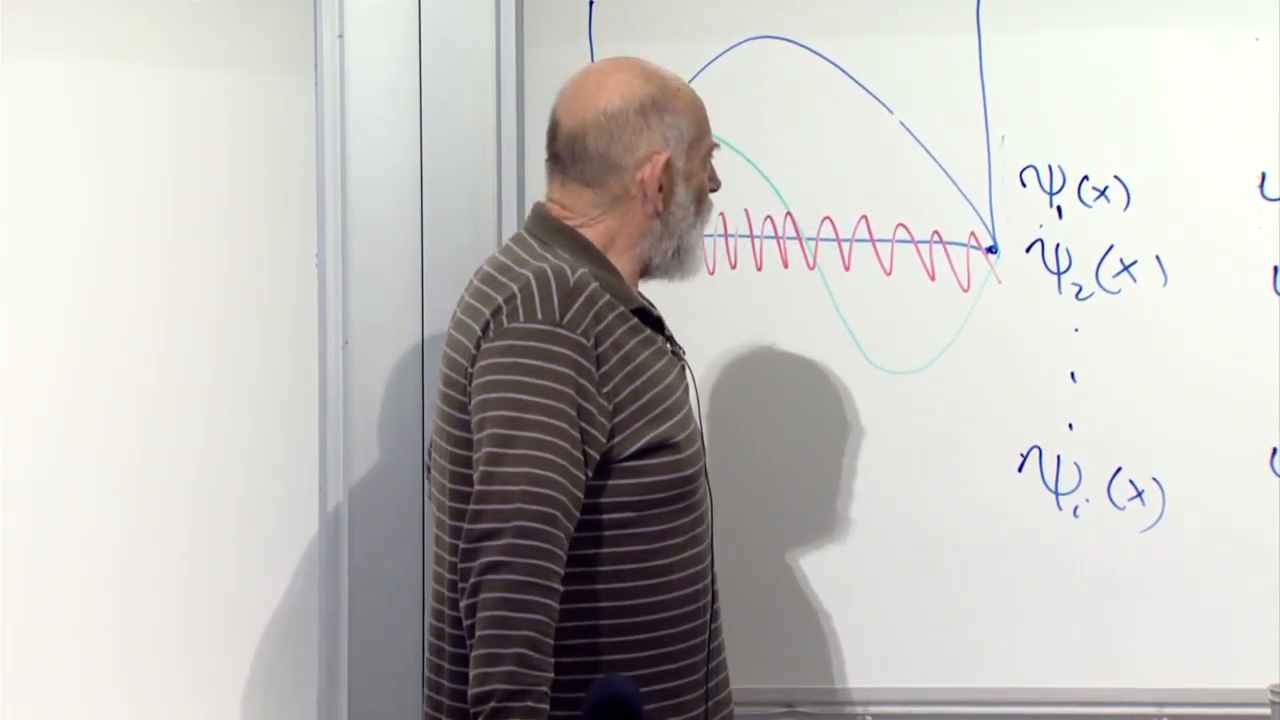
\includegraphics[width=0.9\linewidth]{lecture_06_frame_03.png}
\caption{Одночастичные моды в ящике, упорядоченные по возрастанию энергии. Первая мода не имеет внутренних узлов, вторая имеет один, а опущенные более высокие моды колеблются всё быстрее.}
\lectureframe{00:43:10}
\end{figure}

Ту же структуру можно перерисовать без того перекрытия, которое возникает на доске в аудитории:
\begin{figure}[htbp]
\centering
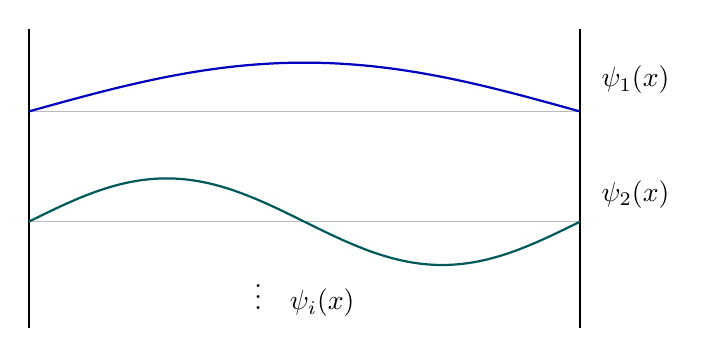
\begin{tikzpicture}[x=1cm,y=1cm]
  \draw[thick] (0,0) -- (0,3.8);
  \draw[thick] (7,0) -- (7,3.8);
  \draw[gray!55] (0,2.75) -- (7,2.75);
  \draw[gray!55] (0,1.35) -- (7,1.35);
  \draw[blue!75!black,thick,domain=0:7,samples=120]
    plot (\x,{2.75+0.62*sin(180*\x/7)});
  \draw[teal!70!black,thick,domain=0:7,samples=120]
    plot (\x,{1.35+0.55*sin(360*\x/7)});
  \node[right] at (7.15,3.15) {$\psi_1(x)$};
  \node[right] at (7.15,1.70) {$\psi_2(x)$};
  \node at (3.5,0.45) {$\vdots\quad \psi_i(x)$};
\end{tikzpicture}
\caption{Аккуратная реконструкция качественного наброска мод в ящике. Смещение по вертикали разделяет собственные функции для удобства чтения и не является дополнительной физической координатой.}
\end{figure}

Индекс \(i\) обозначает одночастичное состояние, а не частицу и не число узлов. В базисе ящика \(i\) оказывается на единицу больше числа внутренних узлов. Каждому состоянию соответствует энергия \(\varepsilon_i\). Следуя обозначениям лекции, мы можем записать эту энергию как \(\hbar\omega_i\), или просто \(\omega_i\) после того, как положено \(\hbar=1\).

\begin{classroomqa}
\lecturetimestamp{00:39:01}
\audiencequestion{Было ли прежнее предположение о независимости точным, и может ли индекс \(i\) обозначать возможные состояния электрона в атоме?}
\lecturerresponse{В построении с независимыми модами коммутация между различными модами точна. Индекс может обозначать одночастичные атомные состояния. Если же частицы взаимодействуют, простой гамильтониан независимых мод уже не исчерпывает всей картины.}
\end{classroomqa}

\begin{classroomqa}
\lecturetimestamp{00:40:34}
\audiencequestion{Является ли частица в ящике бозоном?}
\lecturerresponse{Может, но при одной частице статистика не имеет значения. Запрет и обмен приобретают смысл только тогда, когда имеется более одной тождественной частицы.}
\end{classroomqa}

\section{От мод в ящике к пространству Фока}

Теперь допустим в ящике любое число тождественных бозонов. Некоторое число \(n_1\) может занимать \(\psi_1\), некоторое число \(n_2\) может занимать \(\psi_2\), и так далее. Поэтому базисное состояние имеет вид
\begin{equation}
|n_1,n_2,n_3,\ldots\rangle.
\end{equation}
Это в точности то обозначение, которое уже использовалось для многих осцилляторов. Это тождество носит структурный характер: сопоставим каждому одночастичному состоянию один осциллятор и отождествим число возбуждения осциллятора с числом частиц, занимающих это состояние.

Бозоны здесь существенны, потому что каждое \(n_i\) может быть любым неотрицательным целым числом. Для фермионов каждое одночастичное состояние может быть пустым или занятым одной частицей, но никогда не двумя, так что обычную алгебру осциллятора нельзя использовать без изменений.

Операторы теперь можно определить по их действию на базис чисел заполнения. Оператор \(a_i^\dagger\) создаёт одну частицу в одночастичном состоянии \(i\); \(a_i\) уничтожает одну:
\begin{align}
a_i^\dagger|n_1,\ldots,n_i,\ldots\rangle
&=\sqrt{n_i+1}\,|n_1,\ldots,n_i+1,\ldots\rangle, \\
a_i|n_1,\ldots,n_i,\ldots\rangle
&=\sqrt{n_i}\,|n_1,\ldots,n_i-1,\ldots\rangle.
\end{align}
Это не аналогия, придуманная задним числом. Это и есть определение бозонных операторов рождения и уничтожения на этом базисе. Поскольку этот базис порождает пространство, по линейности определение задаёт их действие на любом состоянии.

\begin{classroomqa}
\lecturetimestamp{00:47:11}
\audiencequestion{Являются ли \(n_1,n_2,n_3\) квантовыми состояниями?}
\lecturerresponse{Метки \(1,2,3,\ldots\) задают одночастичные состояния. Символы \(n_1,n_2,n_3,\ldots\) — это числа частиц, занимающих эти состояния. Главная трудность обозначений состоит в том, чтобы не смешивать метку состояния с его числом заполнения.}
\end{classroomqa}

\subsection{Что делает квадратный корень}

Множитель \(\sqrt{n_i+1}\) не обозначает ни дополнительную частицу, ни отдельный физический процесс. Он обеспечивает оператору правильную нормировку и правильную алгебру. Для одной моды
\begin{align}
a a^\dagger|n\rangle
&=a\bigl(\sqrt{n+1}\,|n+1\rangle\bigr) \\
&=(n+1)|n\rangle,
\end{align}
тогда как
\begin{equation}
a^\dagger a|n\rangle=n|n\rangle.
\end{equation}
Поэтому их разность равна \(|n\rangle\), как и требуется условием \([a,a^\dagger]=1\). Очень грубо говоря, каждый из двух лестничных операторов имеет порядок \(\sqrt n\), поскольку их произведение даёт оператор числа частиц порядка \(n\).

\begin{classroomqa}
\lecturetimestamp{00:47:52}
\audiencequestion{Какой осязаемый физический смысл имеет множитель с квадратным корнем?}
\lecturerresponse{В первую очередь это математическая нормировка. Он обеспечивает, что состояния с числами заполнения нормированы, что \(a^\dagger a\) имеет собственное значение \(n\) и что лестничные операторы удовлетворяют коммутатору осциллятора. Иногда математика и есть тот смысл, который нужен.}
\end{classroomqa}

\begin{classroomqa}
\lecturetimestamp{00:52:25}
\audiencequestion{Были ли операторы рождения и уничтожения определены только через их свойства и их действие на базис?}
\lecturerresponse{Да. Определения не обязаны возникать из более первичной картины. Их ценность проверяется их следствиями. Если задать действие на полном базисе, операторы тем самым задаются на всём пространстве, и эти определения воспроизводят нужные коммутационные соотношения.}
\end{classroomqa}

\begin{classroomqa}
\lecturetimestamp{00:53:22}
\audiencequestion{Почему \(a_i\) заставляет частицу исчезнуть, а не просто переводит её в другое состояние?}
\lecturerresponse{Потому что \(a_i\) по определению понижает заполнение состояния \(i\). Полезный вопрос состоит не в том, почему определение истинно, а в том, почему оно полезно. Оно полезно потому, что испускание и поглощение требуют операторов, меняющих число частиц: фотон создаётся при испускании излучения и уничтожается при его поглощении.}
\end{classroomqa}

Пространство, порождаемое всеми состояниями с числами заполнения, есть \emph{пространство Фока}. Оно содержит вакуум, все одночастичные состояния, все двухчастичные состояния и так далее без фиксированной верхней границы:
\begin{equation}
\mathcal F=\mathcal H_0\oplus\mathcal H_1\oplus\mathcal H_2\oplus\cdots.
\label{eq:l06-fock-space}
\end{equation}
Обозначение прямой суммы явно показывает то, чего обычная \(N\)-частичная волновая функция не показывала: все секторы с разным числом частиц принадлежат одному пространству состояний.

\begin{classroomqa}
\lecturetimestamp{00:54:56}
\audiencequestion{Определяет ли задание операторов на собственных векторах чисел заполнения их действие на произвольные векторы, и следуют ли тогда коммутаторы осциллятора?}
\lecturerresponse{Именно. Векторы заполнения образуют базис, поэтому линейность распространяет определение на всё пространство Фока. Действуя на этом базисе, мы проверяем бозонные коммутационные соотношения. Каждому одночастичному состоянию соответствует один осциллятор, а его число заполнения как осциллятора равно числу частиц в этом состоянии.}
\end{classroomqa}

\subsection{Вакуум и свободный гамильтониан}

Вакуум Фока — это состояние, в котором ни в одном одночастичном состоянии нет частиц:
\begin{equation}
|0\rangle=|0,0,0,\ldots\rangle,
\qquad a_i|0\rangle=0.
\end{equation}
Слово \emph{основное состояние} здесь может вводить в заблуждение. Самое низкое \emph{одночастичное} состояние — это мода \(i=1\); в вакууме Фока нет частицы даже в этой моде. Если частица занимает низшую моду, \(a_1\) может уничтожить её и вернуть систему в вакуум.

\begin{classroomqa}
\lecturetimestamp{00:56:19}
\audiencequestion{Что такое вакуум на языке чисел заполнения? Занято ли низшее одночастичное состояние?}
\lecturerresponse{В вакууме все числа заполнения равны нулю, и он аннулируется каждым \(a_i\). Низшая одночастичная мода в вакууме не занята. Если бы она была занята, её оператор уничтожения мог бы убрать эту частицу.}
\end{classroomqa}

Для невзаимодействующих частиц полная энергия аддитивна. Если одна частица в состоянии \(i\) имеет энергию \(\hbar\omega_i\), то
\begin{align}
H
&=\sum_i \hbar\omega_i N_i \\
&=\sum_i \hbar\omega_i a_i^\dagger a_i.
\label{eq:l06-free-fock-hamiltonian}
\end{align}
Здесь возможны два эквивалентных прочтения. Это сумма энергий осцилляторов, по одному осциллятору на каждое одночастичное состояние. Это также сумма по одночастичным энергиям, каждая из которых умножена на число частиц, обладающих этой энергией.

В обозначениях теории поля \(a_i^\dagger\) обычно называется оператором рождения, а \(a_i\) — оператором уничтожения. Более старое обозначение \(a_+\) и \(a_-\) означает то же самое.

\section{Уточнения перед появлением поля}

Несколько вопросов после перерыва позволяют отличить новую осцилляторную схему учёта от обычной частицы, движущейся в осцилляторном потенциале.

\begin{classroomqa}
\lecturetimestamp{01:06:09}
\audiencequestion{Энергетические уровни частицы в ящике не равноотстоящие, так где же здесь гармонический осциллятор?}
\lecturerresponse{Одночастичные энергии \(\omega_i\) не обязаны быть равноотстоящими. Однако для каждой фиксированной моды \(i\) энергии нуля, одной, двух и трёх невзаимодействующих частиц в этой моде равны \(0,\omega_i,2\omega_i,3\omega_i\). Эта лестница заполнения и есть осциллятор. Она отлична от ситуации, когда одна частица помещена в потенциал гармонического осциллятора.}
\end{classroomqa}

\begin{classroomqa}
\lecturetimestamp{01:08:38}
\audiencequestion{Связано ли это построение с разложением Фурье?}
\lecturerresponse{Самым тесным образом. Если одночастичный базис состоит из мод импульса, то модовые функции — это синусы, косинусы или комплексные экспоненты, а \(a_i\) являются квантовыми аналогами коэффициентов Фурье. Общий базис не обязан быть тригонометрическим, но логика разложения остаётся той же.}
\end{classroomqa}

\begin{classroomqa}
\lecturetimestamp{01:09:07}
\audiencequestion{Всем ли частицам приписывается одна и та же энергия, и учтены ли взаимодействия?}
\lecturerresponse{Частицы, занимающие одно и то же одночастичное состояние, имеют одну и ту же энергию, тогда как частицы в разных состояниях, вообще говоря, имеют разные энергии. Пока частицы свободны: они не взаимодействуют. Взаимодействия добавили бы члены потенциальной энергии, так что гамильтониан уже не был бы просто аддитивной суммой в уравнении~\eqref{eq:l06-free-fock-hamiltonian}.}
\end{classroomqa}

\begin{classroomqa}
\lecturetimestamp{01:10:26}
\audiencequestion{Что стало с половиной кванта энергии нулевых колебаний в каждом осцилляторе?}
\lecturerresponse{Это аддитивная константа в гамильтониане. Константа коммутирует с любым оператором, так что она не изменяет уравнения движения Гейзенберга, а обычные негравитационные измерения зависят от разностей энергий. Для специальных целей она может иметь значение, но на построение, развиваемое здесь, не влияет.}
\end{classroomqa}

Свободная теория уже сама по себе представляет собой аппарат учёта необычайной силы. Она позволяет отслеживать не только множество частиц, но и частицы, которые меняют состояние, появляются, исчезают или существуют в суперпозициях с различным полным числом. Операторы — это не просто символы учёта, поскольку подходящие эрмитовы комбинации можно измерять, но как первая интуиция такой взгляд полезен.

\begin{classroomqa}
\lecturetimestamp{01:14:03}
\audiencequestion{Откуда исторически возникли теория поля и квантовая теория поля?}
\lecturerresponse{Краткий исторический очерк начинается с физической картины электрических и магнитных полей у Фарадея и уравнений Максвелла для классических полей. Планк ввёл кванты энергии при изучении теплового излучения; Эйнштейн отнёс квантование к самому электромагнитному полю и к квантам света. Затем Хайзенберг, Паули и особенно Дирак помогли сформировать современный операторный формализм к концу 1920-х годов. Ультрафиолетовая катастрофа и квантовое описание излучения были среди решающих ранних проблем. Это схематическая история, а не исчерпывающее распределение приоритетов.}
\end{classroomqa}

Эта историческая нить также объясняет, почему осцилляторы всё время возвращаются. Классическое излучение в полости раскладывается по нормальным модам. Квантование этих мод превращает числа их возбуждения в числа фотонов. Математические кванты, занимающие эти моды, становятся физическими частицами.

\section{Оператор бозонного поля}

Пусть \(\{\psi_i(x)\}\) — полный ортонормированный базис одночастичных волновых функций. Определим
\begin{equation}
\boxed{\Psi(x)=\sum_i a_i\,\psi_i(x)}
\label{eq:l06-field-annihilation}
\end{equation}
и его эрмитово сопряжение
\begin{equation}
\boxed{\Psi^\dagger(x)=\sum_i a_i^\dagger\,\psi_i^*(x)}.
\label{eq:l06-field-creation}
\end{equation}

\begin{figure}[htbp]
\centering
\includegraphics[width=0.9\linewidth]{lecture_06_frame_04.png}
\caption{Полные разложения по модам поля уничтожения и его эрмитова сопряжения. Уравнения~\eqref{eq:l06-field-annihilation} и \eqref{eq:l06-field-creation} сохраняют в наборе ту же структуру операторов и комплексного сопряжения.}
\lectureframe{01:25:15}
\end{figure}

Для любого фиксированного положения \(x\) каждое \(\psi_i(x)\) — обычное комплексное число. Всё операторное содержание заключено в \(a_i\) и \(a_i^\dagger\). Когда \(x\) меняется, мы получаем другой оператор в каждой точке пространства. Именно в этом точном смысле \(\Psi\) является операторнозначной функцией.

Если базисные функции — плоские волны, то уравнения~\eqref{eq:l06-field-annihilation} и \eqref{eq:l06-field-creation} представляют собой квантовые разложения Фурье: классические коэффициенты Фурье стали операторами. В ящике базисом вместо этого могут служить синусные функции из уравнения~\eqref{eq:l06-box-basis}. Подходит любой полный ортонормированный одночастичный базис.

Ни \(\Psi\), ни \(\Psi^\dagger\) не является эрмитовым. Наблюдаемые поля можно строить из эрмитовых комбинаций, таких как
\begin{equation}
\Psi(x)+\Psi^\dagger(x),
\qquad
i\bigl(\Psi^\dagger(x)-\Psi(x)\bigr),
\end{equation}
а наблюдаемые плотности позже будут строиться из произведений, таких как \(\Psi^\dagger(x)\Psi(x)\). Сейчас задача прежде всего понять, что делают два базовых поля.

\begin{classroomqa}
\lecturetimestamp{01:23:14}
\audiencequestion{Как левая часть может быть оператором, если модовые функции справа — обычные волновые функции?}
\lecturerresponse{Функции \(\psi_i(x)\) после выбора \(x\) являются числами. Множители \(a_i\) — операторы. Число, умноженное на оператор, даёт оператор, и потому сумма тоже является оператором. Изменяя \(x\), мы получаем всё семейство операторов.}
\end{classroomqa}

\section{Что делает поле}

Поле уничтожения сразу уничтожает вакуум:
\begin{equation}
\Psi(x)|0\rangle
=\sum_i\psi_i(x)a_i|0\rangle
=0.
\label{eq:l06-field-kills-vacuum}
\end{equation}
Поле рождения делает нечто гораздо более содержательное.

Пусть \(|i\rangle\) обозначает одночастичное состояние с волновой функцией
\begin{equation}
\langle x|i\rangle=\psi_i(x).
\end{equation}
Из полноты одночастичного базиса следует
\begin{equation}
\sum_i|i\rangle\langle i|=1.
\label{eq:l06-completeness}
\end{equation}
Применим это тождество к собственному состоянию координаты:
\begin{align}
|x\rangle
&=\sum_i|i\rangle\langle i|x\rangle \\
&=\sum_i\psi_i^*(x)|i\rangle.
\label{eq:l06-position-expansion}
\end{align}
На языке Фока одночастичное модовое состояние имеет вид
\begin{equation}
|i\rangle=a_i^\dagger|0\rangle.
\end{equation}
Подставляя это в уравнение~\eqref{eq:l06-position-expansion},
\begin{align}
|x\rangle
&=\sum_i\psi_i^*(x)a_i^\dagger|0\rangle \\
&=\Psi^\dagger(x)|0\rangle.
\label{eq:l06-local-creation}
\end{align}
Следовательно, \(\Psi^\dagger(x)\) создаёт частицу, локализованную в точке \(x\), тогда как \(\Psi(x)\) удаляет там одну частицу. Собственное состояние координаты локализовано дельта-функцией и является обобщённым, ненормируемым состоянием; физическую локализованную частицу получают, свёртывая поле с нормируемым волновым пакетом.\editorialnote{В лекции используется идеализированный язык собственных состояний координаты. Уточнение о волновом пакете фиксирует стандартный математический смысл, не изменяя аргумента.}

\begin{classroomqa}
\lecturetimestamp{01:36:26}
\audiencequestion{Где содержится информация о том, какого вида частица создаётся? Является ли состояние в \(x\) локализованным дельта-функцией?}
\lecturerresponse{Каждому виду частиц сопоставляется отдельное поле, так что тождество частицы задаётся тем, какое поле используется. Аргумент \(x\) указывает, где она создаётся. В идеальном координатном базисе создаваемое состояние дельта-функционально локализовано.}
\end{classroomqa}

К примерам бозонных видов относятся фотоны, гравитоны, бозоны Хиггса и глюоны, хотя реалистические поля также несут внутренние индексы. Даже для фотонов нужны поляризационные метки. Упрощённая нотация скалярного поля опускает эти дополнительные метки, чтобы сам принцип создания оставался наглядным.

\subsection{Вакуум — не нулевой вектор}

Уравнение
\begin{equation}
\Psi(x)|0\rangle=0
\end{equation}
содержит два очень разных объекта, обозначаемых нулём. Кет \(|0\rangle\) — это вакуум: нормированное физическое состояние, для которого
\begin{equation}
\langle0|0\rangle=1.
\end{equation}
Результат справа — нулевой вектор. Его норма равна нулю; его нельзя нормировать, и он не представляет физического состояния.

Различие становится особенно ясным при сложении. Прибавление нулевого вектора к одночастичному состоянию ничего не меняет. Прибавление вакуума к одночастичному состоянию даёт настоящую суперпозицию секторов с разным числом частиц. При нормированных коэффициентах
\begin{equation}
|\chi\rangle=\frac{1}{\sqrt2}\bigl(|0\rangle+|1\rangle\bigr)
\end{equation}
имеет равные вероятности состояний с нулём и с одной частицей. Это не то же самое, что \(|1\rangle\).

\begin{classroomqa}
\lecturetimestamp{01:37:23}
\audiencequestion{Если в \(x\) нет частицы, не делает ли \(\Psi(x)\) просто ничего? Что означает, что результат равен нулю?}
\lecturerresponse{Нет, исходное состояние не возвращается. Результатом является нулевой вектор. Вакуум — это нормированное состояние, описывающее пустое пространство; нулевой вектор имеет нулевую длину и не описывает никакого физического состояния. Любой оператор, действуя на нулевой вектор, возвращает нулевой вектор.}
\end{classroomqa}

\begin{classroomqa}
\lecturetimestamp{01:39:00}
\audiencequestion{Что происходит, если к одночастичному состоянию прибавить вакуум, а не нулевой вектор?}
\lecturerresponse{Получается суперпозиция с амплитудами для разных чисел частиц. Напротив, прибавление нулевого вектора оставляет одночастичное состояние неизменным. Символ в \(|0\rangle\) обозначает нулевое заполнение; он не означает нулевой вектор.}
\end{classroomqa}

\begin{classroomqa}
\lecturetimestamp{01:41:56}
\audiencequestion{Имеет ли значение порядок модовой функции и её оператора рождения или уничтожения в разложении поля? Являются ли модовые функции комплексными?}
\lecturerresponse{Модовая функция — обычное число и потому коммутирует с любым оператором, так что порядок не имеет значения. Вообще говоря, модовые функции могут быть комплексными; будет ли выбранный базис вещественным или комплексным, зависит от одночастичной задачи Schr\"odinger.}
\end{classroomqa}

\subsection{Две частицы и возникновение бозонной симметрии}

Чтобы создать одну частицу в \(x\) и другую в \(y\), нужно подействовать дважды:
\begin{equation}
|x,y\rangle
=\Psi^\dagger(y)\Psi^\dagger(x)|0\rangle.
\label{eq:l06-two-particle-state}
\end{equation}
Эти точки могут совпадать или различаться. Поскольку лежащие в основе операторы рождения коммутируют,
\begin{align}
[\Psi^\dagger(x),\Psi^\dagger(y)]
&=\sum_{i,j}\psi_i^*(x)\psi_j^*(y)
[a_i^\dagger,a_j^\dagger] \\
&=0.
\end{align}
отсюда следует, что
\begin{equation}
\Psi^\dagger(y)\Psi^\dagger(x)|0\rangle
=\Psi^\dagger(x)\Psi^\dagger(y)|0\rangle.
\label{eq:l06-boson-exchange}
\end{equation}
Перестановка порядка двух частиц ничего не меняет. Это и есть бозонная обменная симметрия. Поэтому мы могли бы начать с алгебры осциллятора и \emph{вывести}, что частицы, построенные из коммутирующих операторов рождения, являются бозонами. Для фермионов вместо этого потребуются антикоммутирующие операторы.

\begin{classroomqa}
\lecturetimestamp{01:42:37}
\audiencequestion{Как добавить вторую частицу к одночастичному состоянию?}
\lecturerresponse{Примените ещё одно поле рождения. Чтобы добавить её в \(y\), подействуйте \(\Psi^\dagger(y)\) слева от \(\Psi^\dagger(x)\). Результатом будет двухчастичное состояние из уравнения~\eqref{eq:l06-two-particle-state}.}
\end{classroomqa}

\begin{classroomqa}
\lecturetimestamp{01:46:04}
\audiencequestion{Полностью ли эквивалентна коммутативность двух полей рождения симметризации двухчастичного состояния?}
\lecturerresponse{Да. Она делает состояние с одной частицей в \(x\) и одной в \(y\) тождественным состоянию, полученному после обмена меток. Это определяющее обменное свойство тождественных бозонов.}
\end{classroomqa}

\begin{classroomqa}
\lecturetimestamp{01:46:32}
\audiencequestion{Означает ли это, что частицы в точках \(x\) и \(y\) должны быть бозонами одного и того же вида?}
\lecturerresponse{Да. Аргументы \(x\) и \(y\) — это координаты, тогда как одно поле описывает один вид частиц. Для различных видов, а также для дополнительных меток, таких как две поляризации фотона, требуются отдельные компоненты поля.}
\end{classroomqa}

\section{Почему важно переменное число частиц}

Если бы в задаче всегда было ровно 37 частиц, язык полей был бы лишь необязательным средством учёта. Его подлинная сила проявляется, когда частицы могут испускаться и поглощаться, и особенно когда само число частиц является квантовой переменной. Пространство Фока допускает состояния вида
\begin{equation}
|\Phi\rangle
=c_0|0\rangle+c_1|1\rangle+c_2|2\rangle+\cdots,
\qquad
\sum_{n=0}^{\infty}|c_n|^2=1.
\end{equation}
Важный пример — лазерное поле: вообще говоря, это не состояние с одним точно определённым числом фотонов, а суперпозиция многих секторов с различным числом фотонов.

Теперь связь между частицами и полями выражена явно. Операторы мод подсчитывают частицы в собственных состояниях энергии и изменяют их число; поле объединяет эти операторы с полным набором волновых функций, так что частицы можно создавать или уничтожать в заданных точках. Алгебра гармонических осцилляторов стала элементарным языком бозонного квантового поля.
